\documentclass{article} % say
\usepackage{tikz}
\begin{document}
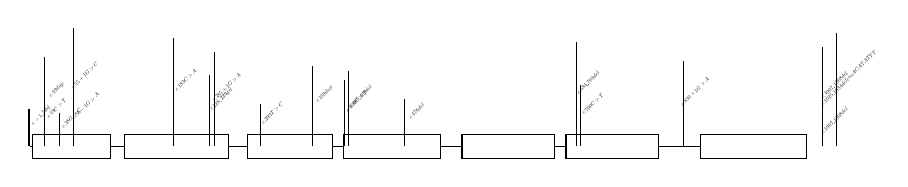
\begin{tikzpicture}[scale=0.03]
    % Draw protein domain 
    % domain width, found at https://www.uniprot.org/uniprot/Q9Y484
    \def\domains{ 1/34, 40/84, 92/128, 133/174, 183/222, 227/266, 284/329}
    \def\h{5}
    \foreach \s / \e in \domains {
        \draw (\s, -\h) rectangle (\e, \h);
    }
    % Draw links
    \foreach \s/\e [remember=\e as \laste (initially 0)] in \domains {
        \draw (\laste, 0) -- (\s, 0);
    }
    \def\variants{
1007/c.1007\_1008del
, 38/c.38G>C
, -1/c.-1\_5del
, 293/c.293T>C
, 476/c.476del
, 19/c.19C>T
, 56/c.56-1G>A
, 700/c.700C>T
, 400/c.400C>T
, 228/c.228\_229del
, 405/c.405\_409del
, 359/c.359dup
, 830/c.830+1G>A
, 19/c.19dup
, 235/c.235+1G>A
, 1007/c.1007\_1008del
, 694/c.694\_703del
, 183/c.183C>A
, 1025/c.1025\_1034delinsACATATTT
,     55/c.55+1G>C}

\foreach \v/\t [count=\i] in \variants{
    \draw (\v/3,0) -- (\v/3, 2*\h+2*\i); 
    \draw  (\v/3+5, 2*\h+\i) node [rotate=45, scale=0.2] {$\t$}; 
}

\end{tikzpicture}
\end{document}
